\chapter{Secure Cloud Deployment Framework (SCDF)}
\label{chap:third}

\ifpdf
    \graphicspath{{Chapter3/Figures/PNG/}{Chapter3/Figures/PDF/}{Chapter3/Figures/}}
\else
    \graphicspath{{Chapter3/Figures/EPS/}{Chapter3/Figures/}}
\fi

% ----------------------------------------------------------
\section{Chapter Overview and Positioning}
\label{sec:chapter3_overview}

This chapter translates the findings of the Systematic Literature Review (SLR) presented in Chapter~\ref{chap:second} into a practical, evidence-driven Secure Cloud Deployment Framework (SCDF). The framework is designed for Small and Medium Enterprises (SMEs) operating primarily on Infrastructure-as-a-Service (IaaS) platforms, particularly in developing or resource-constrained environments.

The synthesis of empirical evidence from the literature revealed a persistent disconnect: SMEs recognize the necessity of cloud adoption but lack actionable guidance for deploying cloud infrastructure securely under constraint. Existing frameworks and standards---while comprehensive---were developed for enterprise contexts with mature governance structures, dedicated security teams, and substantial budgets. SCDF addresses this gap by providing a minimal, deployable, and risk-driven framework that targets the dominant failure modes identified in the literature: misconfiguration, skills shortages, and reactive security postures.

SCDF is not intended to replace established security standards such as ISO/IEC~27001 or NIST SP~800-53, nor does it claim to achieve formal compliance certification. Instead, it operationalizes security principles into concrete, sequenced actions that SMEs can implement with limited resources. The framework prioritizes foundational security controls that address the most common threat vectors---identity compromise, network exposure, and configuration drift---while remaining compatible with incremental maturity growth as organizational capacity improves.

% ----------------------------------------------------------
\section{Scope Definition and Applicability Boundaries}
\label{sec:scope_definition}

\subsection{Target SME Profile}
\label{subsec:target_sme_profile}

SCDF is designed for SMEs that exhibit most or all of the following characteristics:

\begin{itemize}
    \item \textbf{Organizational scale:} Typically fewer than 250 employees, with limited or non-existent dedicated cybersecurity personnel.
    \item \textbf{Technical capacity:} Reliance on external IT support providers, part-time technical staff, or small internal IT teams without specialized security expertise.
    \item \textbf{Cloud consumption model:} Primary use of Infrastructure-as-a-Service (IaaS) including virtual machines, block storage, object storage, and basic networking; minimal deployment of complex Platform-as-a-Service (PaaS) or container orchestration platforms.
    \item \textbf{Economic constraints:} High cost sensitivity and preference for free, open-source, or freemium tooling over commercial enterprise security solutions.
    \item \textbf{Operational reality:} Deployment in environments characterized by intermittent connectivity, limited management bandwidth, and competing business priorities that may defer security investment.
\end{itemize}

This profile represents the modal SME in developing regions---organizations for whom cloud adoption is structurally necessary but whose operational constraints render conventional enterprise frameworks inapplicable without significant adaptation.

\subsection{Explicit Exclusions}
\label{subsec:explicit_exclusions}

To maintain feasibility and realism, SCDF deliberately excludes the following capabilities and objectives:

\begin{itemize}
    \item \textbf{Formal certification pursuit:} SCDF does not prescribe controls or documentation processes sufficient for formal ISO/IEC~27001, SOC~2, or other compliance certifications. While alignment with these standards is acknowledged, certification attainment exceeds the resource capacity of the target profile.
    \item \textbf{Enterprise-scale Zero Trust:} Full Zero Trust architectures requiring pervasive micro-segmentation, dynamic authorization policies, and continuous device attestation are excluded. SCDF implements risk-appropriate identity and network controls that represent Zero Trust principles without architectural complexity.
    \item \textbf{Security Operations Center (SOC):} 24/7 threat hunting, dedicated incident response teams, and continuous human monitoring are beyond scope. SCDF emphasizes automated detection with targeted human response.
    \item \textbf{Cloud provider obligation substitution:} SCDF supplements but does not replace provider shared-responsibility obligations. Physical security, hypervisor integrity, and underlying infrastructure remain provider responsibilities.
\end{itemize}

These exclusions are not limitations but intentional boundaries that ensure the framework remains deployable within real-world SME constraints.

% ----------------------------------------------------------
\section{Derivation of Framework Requirements from SLR Findings}
\label{sec:derivation_requirements}

The design of SCDF is systematically derived from the synthesized findings of the systematic literature review. Table~\ref{tab:slr_to_requirements} maps each major SLR finding to an identified constraint and the corresponding SCDF requirement.

\begin{table}[htbp]
    \centering
    \caption{Mapping SLR Findings to SCDF Requirements}
    \label{tab:slr_to_requirements}
    \resizebox{\textwidth}{!}{%
    \begin{tabular}{|p{5cm}|p{4cm}|p{5cm}|}
        \hline
        \textbf{SLR Finding} & \textbf{Identified Constraint} & \textbf{SCDF Requirement} \\
        \hline
        Misconfiguration is the dominant cause of cloud security incidents & Limited expertise and human error & Secure-by-default baselines and automated configuration validation \\
        \hline
        Skills gap exceeds tooling availability & Lack of trained security personnel & Guided workflows with constrained decision spaces \\
        \hline
        Cost is a primary adoption barrier & Severe budget limitations & Preference for OSS, freemium, or native cloud controls; explicit trade-off documentation \\
        \hline
        Connectivity instability affects availability and monitoring & Unreliable network infrastructure & Fail-safe and asynchronous security controls; local-first resilience \\
        \hline
        Existing frameworks are too abstract or complex & Low operational applicability for SMEs & Concrete control mapping and step-by-step workflows \\
        \hline
        Reactive rather than proactive security posture & Limited monitoring capability & Automated detection with prioritized alerting \\
        \hline
    \end{tabular}%
    }
\end{table}

\subsection{Validation of Requirements}

Each derived requirement addresses a documented failure mode from the literature. For example, the requirement for secure-by-default baselines responds directly to findings that SMEs frequently deploy with default configurations due to lack of implementation guidance \citep{Milhem2025integrated,Gibreel2023Factors}. Similarly, the preference for open-source tooling addresses the economic constraints identified across multiple regional studies \citep{Skafi2020Factors,Wilson2015Enablers,Sayginer2021Multi}.

% ----------------------------------------------------------
\section{Design Principles and Trade-Off Rationale}
\label{sec:design_principles}

\subsection{Core Design Principles}
\label{subsec:core_principles}

SCDF is governed by five core design principles that prioritise deployability over comprehensiveness:

\begin{enumerate}
    \item \textbf{Risk-driven prioritization:} Controls are sequenced by threat frequency and impact. Identity compromise, network exposure, and unpatched vulnerabilities---the three most common initial access vectors for SMEs---are addressed before less common vectors.
    
    \item \textbf{Minimal viable security:} The framework implements essential controls rather than exhaustive coverage. A partially implemented SCDF deployment covering identity and network security provides more risk reduction than a comprehensive framework that remains unimplemented due to complexity.
    
    \item \textbf{Automation as compensation:} Automation compensates for limited human expertise by enforcing consistency and reducing configuration drift. However, automation does not eliminate governance requirements---human oversight remains essential for approval gates and incident decision-making.
    
    \item \textbf{Incremental maturity:} SCDF is structured as four progressive phases, allowing SMEs to achieve baseline security and then selectively mature controls as resources permit. There is no binary pass/fail; partial implementation is explicitly supported.
    
    \item \textbf{Provider-agnostic with pragmatic exceptions:} Core controls are portable across major IaaS providers, but vendor-specific native tools are permitted where they reduce cost or complexity without compromising security.
\end{enumerate}

\subsection{Explicit Trade-Offs}
\label{subsec:explicit_tradeoffs}

The design of SCDF requires explicit acceptance of trade-offs that prioritize feasibility:

\begin{itemize}
    \item \textbf{Breadth \textit{versus} deployability:} SCDF sacrifices comprehensive coverage of all potential threat vectors in favor of deployable, executable guidance for the most common vectors.
    \item \textbf{Advanced \textit{versus} baseline protection:} Sophisticated controls (e.g., behavioral analytics, custom threat detection rules) are deferred in favor of foundational controls (e.g., MFA, least-privilege access, network segmentation).
    \item \textbf{Vendor neutrality \textit{versus} pragmatic efficiency:} While the framework maintains provider-agnostic core principles, the use of platform-specific native controls is explicitly permitted where implementation effort is reduced.
\end{itemize}

These trade-offs are documented to inform security decisions rather than obscure them. SMEs adopting SCDF should understand what is included and, critically, what remains their responsibility beyond the framework scope.

% ----------------------------------------------------------
\section{Conceptual Structure of the SCDF}
\label{sec:conceptual_structure}

\subsection{Framework Layers}
\label{subsec:framework_layers}

SCDF is organized into three conceptual layers that separate governance from technical implementation, as illustrated in Figure~\ref{fig:scdf_layers}.

\begin{figure}[htbp]
    \centering
    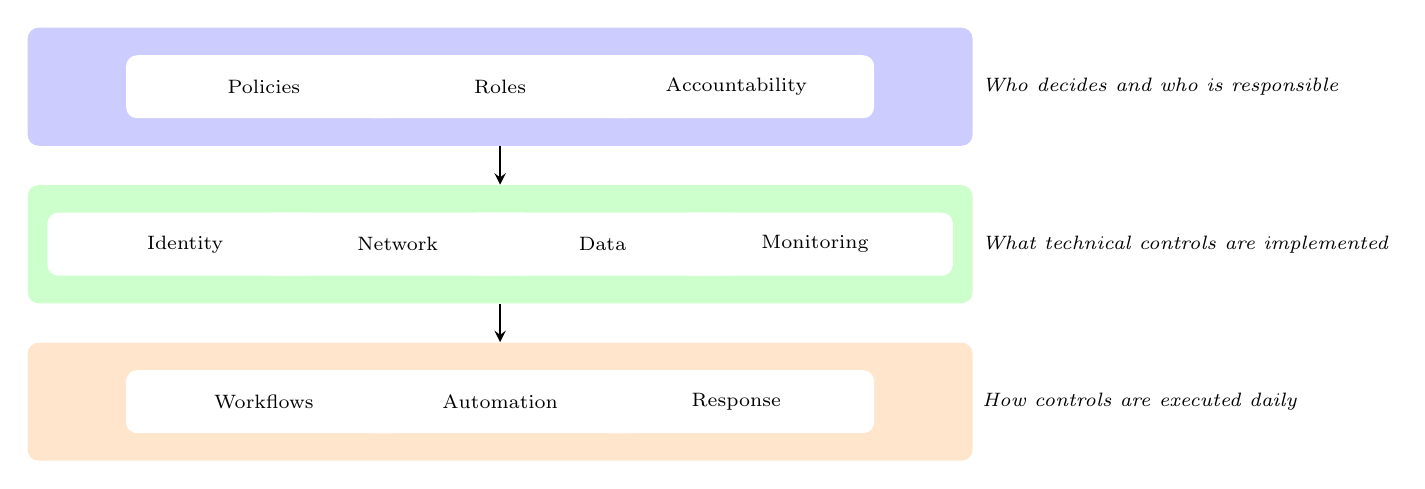
\begin{tikzpicture}[
        layer/.style={rectangle, rounded corners, minimum width=12cm, minimum height=1.5cm, text centered, font=\small\bfseries},
        subelement/.style={rectangle, rounded corners, minimum width=3.5cm, minimum height=0.8cm, text centered, font=\scriptsize, fill=white},
        arrow/.style={->, >=stealth, thick}
    ]
        % Governance Layer
        \node[layer, fill=blue!20] (gov) at (0,4) {Governance Layer};
        \node[subelement] at (-3,4) {Policies};
        \node[subelement] at (0,4) {Roles};
        \node[subelement] at (3,4) {Accountability};
        
        % Control Layer
        \node[layer, fill=green!20] (ctrl) at (0,2) {Control Layer};
        \node[subelement] at (-4,2) {Identity};
        \node[subelement] at (-1.3,2) {Network};
        \node[subelement] at (1.3,2) {Data};
        \node[subelement] at (4,2) {Monitoring};
        
        % Operational Layer
        \node[layer, fill=orange!20] (ops) at (0,0) {Operational Layer};
        \node[subelement] at (-3,0) {Workflows};
        \node[subelement] at (0,0) {Automation};
        \node[subelement] at (3,0) {Response};
        
        % Arrows
        \draw[arrow] (gov) -- (ctrl);
        \draw[arrow] (ctrl) -- (ops);
        
        % Side labels
        \node[right, font=\scriptsize\itshape] at (6,4) {Who decides and who is responsible};
        \node[right, font=\scriptsize\itshape] at (6,2) {What technical controls are implemented};
        \node[right, font=\scriptsize\itshape] at (6,0) {How controls are executed daily};
    \end{tikzpicture}
    \caption{SCDF Three-Layer Architecture}
    \label{fig:scdf_layers}
\end{figure}

SCDF is organized into three conceptual layers that separate governance from technical implementation:

\begin{enumerate}
    \item \textbf{Governance Layer:} Defines policies, assigns roles and accountability, and establishes decision authority. This layer addresses the ``who decides'' and ``who is responsible'' questions without prescribing specific technical implementations.
    
    \item \textbf{Control Layer:} Specifies technical and procedural security controls organized by security domain (identity, network, data, compute, monitoring). Each control includes purpose, implementation options, and verification methods.
    
    \item \textbf{Operational Layer:} Provides executable workflows, automation scripts, and response procedures that translate controls into day-to-day operations.
\end{enumerate}

This layered structure allows SMEs to implement governance and controls independently of operational capacity, recognizing that some organizations may have policy maturity without implementation capability, while others may implement controls without documented governance.

\subsection{Deployment Phases}
\label{subsec:deployment_phases}

Implementation follows four sequential phases, each building on the previous, as shown in Figure~\ref{fig:deployment_phases}.

\begin{figure}[htbp]
    \centering
    \begin{tikzpicture}[
        phase/.style={rectangle, rounded corners, minimum width=3cm, minimum height=1.5cm, text centered, align=center, font=\small\bfseries, draw, thick},
        arrow/.style={->, >=stealth, very thick},
        focus/.style={font=\scriptsize, align=center, text width=3cm}
    ]
        % Phase boxes
        \node[phase, fill=blue!15] (p1) at (0,0) {Phase 1\\Baseline};
        \node[phase, fill=green!15] (p2) at (4,0) {Phase 2\\Hardening};
        \node[phase, fill=orange!15] (p3) at (8,0) {Phase 3\\Monitoring};
        \node[phase, fill=red!15] (p4) at (12,0) {Phase 4\\Recovery};
        
        % Arrows
        \draw[arrow] (p1) -- (p2);
        \draw[arrow] (p2) -- (p3);
        \draw[arrow] (p3) -- (p4);
        
        % Focus areas
        \node[focus, below=0.5cm of p1] {Identity\\Network\\Logging};
        \node[focus, below=0.5cm of p2] {Config Standards\\Vulnerability Mgmt\\Access Control};
        \node[focus, below=0.5cm of p3] {SIEM\\Alerting\\Audit};
        \node[focus, below=0.5cm of p4] {Backups\\Recovery Plans\\Continuity};
        
        % Risk reduction indicator
        \node[above=1cm of p2, font=\small, align=center] {\textbf{Risk Reduction Priority}\\(Highest \textrightarrow Lower)};
    \end{tikzpicture}
    \caption{SCDF Four-Phase Deployment Sequence}
    \label{fig:deployment_phases}
\end{figure}

Implementation follows four sequential phases, each building on the previous:

\begin{enumerate}
    \item \textbf{Phase 1: Baseline Establishment} --- Secure the foundation including identity management, network boundaries, and initial logging.
    
    \item \textbf{Phase 2: Risk Hardening} --- Implement configuration standards, vulnerability management, and access controls.
    
    \item \textbf{Phase 3: Monitoring and Detection} --- Deploy continuous monitoring, alerting, and audit capabilities.
    
    \item \textbf{Phase 4: Backup, Recovery, and Continuity} --- Ensure resilience through automated backups and documented recovery procedures.
\end{enumerate}

These phases are ordered by risk reduction per unit effort. Phase 1 controls (identity and network) address the highest-impact threat vectors and therefore take priority over Phase 4 controls (backup and recovery), despite the importance of both.

% ----------------------------------------------------------
\section{Operational Workflow and Responsibility Model}
\label{sec:operational_workflow}

\subsection{Actor Roles}
\label{subsec:actor_roles}

SCDF recognizes three primary actors in SME cloud security:

\begin{itemize}
    \item \textbf{SME Owner / Management:} Holds ultimate accountability for risk acceptance and business prioritization. Decides security investment levels and accepts residual risk where full mitigation is infeasible.
    
    \item \textbf{Technical Operator:} Implements and maintains controls. May be internal IT staff, external managed service provider, or part-time administrator. Responsible for execution, not strategic risk decisions.
    
    \item \textbf{Automated Systems:} Enforce configuration, conduct monitoring, generate alerts, and execute approved automated responses (e.g., IP blocking, backup initiation).
\end{itemize}

This separation clarifies that while technical operators implement controls, risk decisions remain with accountable management.

\subsection{Decision versus Automation Boundary}
\label{subsec:decision_boundary}

SCDF distinguishes between activities suitable for automation and those requiring human judgment:

\begin{itemize}
    \item \textbf{Automated (no human latency):} Configuration validation, scheduled backups, routine log aggregation, basic pattern-based alerting.
    
    \item \textbf{Human-driven (requires judgment):} Access approval for privileged accounts, incident escalation after initial detection, recovery decision-making during outages, policy exceptions.
\end{itemize}

This boundary ensures that automation reduces routine burden without displacing essential human oversight where judgment is required.

% ----------------------------------------------------------
\section{Tooling and Control Mapping}
\label{sec:tooling_mapping}

\subsection{Tool Selection Criteria}
\label{subsec:tool_selection_criteria}

All tool recommendations in SCDF satisfy the following criteria, as illustrated in Figure~\ref{fig:tool_taxonomy}:

\begin{figure}[htbp]
    \centering
    \begin{tikzpicture}[
        box/.style={rectangle, rounded corners, minimum width=2.5cm, minimum height=0.8cm, text centered, font=\scriptsize, draw, thick},
        criterion/.style={ellipse, minimum width=3cm, minimum height=1cm, text centered, align=center, font=\small\bfseries, fill=blue!10, draw},
        arrow/.style={->, >=stealth}
    ]
        % Central SME node
        \node[criterion, fill=blue!20] (sme) at (0,0) {SME\\Constraints};

        % Four criteria
        \node[criterion] (cost) at (-4,2) {Cost Access};
        \node[criterion] (complex) at (4,2) {Complexity};
        \node[criterion] (maint) at (-4,-2) {Maintenance};
        \node[criterion] (compat) at (4,-2) {Compatibility};

        % Tool examples
        \node[box, fill=green!10] at (-4,3.2) {Free/OSS/Freemium};
        \node[box, fill=green!10] at (4,3.2) {No Security Expertise};
        \node[box, fill=green!10] at (-4,-3.2) {Active Community};
        \node[box, fill=green!10] at (4,-3.2) {Multi-Cloud};

        % Arrows
        \draw[arrow] (sme) -- (cost);
        \draw[arrow] (sme) -- (complex);
        \draw[arrow] (sme) -- (maint);
        \draw[arrow] (sme) -- (compat);
    \end{tikzpicture}
    \caption{SCDF Tool Selection Criteria}
    \label{fig:tool_taxonomy}
\end{figure}

\begin{enumerate}
    \item \textbf{Cost accessibility:} Free, open-source, or freemium with sufficient capability for SME-scale deployments.
    \item \textbf{Complexity appropriateness:} Deployable by generalist IT staff without specialized security expertise.
    \item \textbf{Maintenance sustainability:} Active project with community or vendor support; not deprecated or abandonware.
    \item \textbf{Provider compatibility:} Functional across multiple IaaS platforms or clearly scoped to specific compatible platforms.
\end{enumerate}

\subsection{Identity and Access Management (IAM)}
\label{subsec:iam_tools}

Table~\ref{tab:iam_tools} lists IAM tooling options categorized by deployment phase and implementation effort.

\begin{table}[htbp]
    \centering
    \caption{SCDF IAM Tooling Options by Phase}
    \label{tab:iam_tools}
    \resizebox{\textwidth}{!}{%
    \begin{tabular}{|l|p{5cm}|l|l|l|}
        \hline
        \textbf{Tool/Service} & \textbf{Purpose} & \textbf{Phase} & \textbf{Effort} & \textbf{Cost} \\
        \hline
        Native Cloud IAM & Provider-managed identity (AWS IAM, Azure AD, GCP IAM, OCI IAM, etc.) & P1 & Low & Included \\
        \hline
        MFA (Native/TOTP) & Multi-factor authentication using authenticator apps & P1 & Low & Free \\
        \hline
        Keycloak & Self-hosted SSO and identity federation & P2 & Medium & OSS \\
        \hline
        Auth0 & SaaS authentication and authorization platform & P2 & Low & Freemium \\
        \hline
        Authelia & Lightweight SSO for self-hosted apps & P3 & Medium & OSS \\
        \hline
    \end{tabular}%
    }
\end{table}

\textbf{Critical Control:} Phase 1 must implement MFA for all privileged accounts before any additional hardening.

\subsection{Network and Edge Protection}
\label{subsec:network_tools}

Table~\ref{tab:network_tools} presents network protection tooling organized by deployment phase.

\begin{table}[htbp]
    \centering
    \caption{SCDF Network Protection Tooling by Phase}
    \label{tab:network_tools}
    \resizebox{\textwidth}{!}{%
    \begin{tabular}{|l|p{5cm}|l|l|l|}
        \hline
        \textbf{Tool/Service} & \textbf{Purpose} & \textbf{Phase} & \textbf{Effort} & \textbf{Cost} \\
        \hline
        Security Groups & Instance-level and subnet-level network access control & P1 & Low & Included \\
        \hline
        Network ACLs & Subnet-level stateless traffic filtering & P1 & Low & Included \\
        \hline
        Cloudflare (Free) & Edge WAF, DDoS protection, DNS security & P2 & Low & Freemium \\
        \hline
        Native Provider WAF & Application-layer attack filtering & P2 & Medium & Usage-based \\
        \hline
        OpenSnitch/Portmaster & Host-level application firewall & P3 & Medium & OSS \\
        \hline
        WireGuard/Tailscale & Modern VPN for secure access & P2 & Low & OSS \\
        \hline
    \end{tabular}%
    }
\end{table}

\textbf{Critical Control:} Default-deny security groups must be established in Phase 1, with explicit allow rules only for required services.

\subsection{Configuration Hardening and Audit}
\label{subsec:hardening_tools}

Table~\ref{tab:hardening_tools} lists configuration assessment tools mapped to deployment phases. These tools address the misconfiguration risk identified as the dominant cause of cloud security incidents in the SLR.

\begin{table}[htbp]
    \centering
    \caption{SCDF Configuration Hardening Tooling by Phase}
    \label{tab:hardening_tools}
    \resizebox{\textwidth}{!}{%
    \begin{tabular}{|l|p{4.5cm}|l|l|p{3cm}|}
        \hline
        \textbf{Tool/Service} & \textbf{Purpose} & \textbf{Phase} & \textbf{Effort} & \textbf{Coverage} \\
        \hline
        Prowler & Multi-cloud security posture assessment & P2 & Medium & AWS, Azure, GCP \\
        \hline
        ScoutSuite & Multi-cloud security auditing & P2 & Medium & AWS, Azure, GCP, Alibaba \\
        \hline
        CloudSploit & Continuous cloud security monitoring & P3 & Low & Multi-cloud \\
        \hline
        CIS Benchmarks & Industry-standard configuration guidance & P2 & High & All major IaaS \\
        \hline
        CIS-CAT Lite & Automated configuration assessment & P3 & Medium & Standardized \\
        \hline
        Lynis & Host-level security auditing & P2 & Low & Linux/Unix systems \\
        \hline
        OpenSCAP & Automated compliance checking & P3 & Medium & SCAP-compliant systems \\
        \hline
    \end{tabular}%
    }
\end{table}

\textbf{Automation Priority:} Weekly automated Prowler/ScoutSuite scans should be scheduled in Phase 3, with findings routed to designated response personnel.

\subsection{Monitoring and Logging}
\label{subsec:monitoring_tools}

Table~\ref{tab:monitoring_tools} presents monitoring and logging tooling critical for detecting the anomalous activity and misconfigurations that SLR findings identified as common initial attack vectors.

\begin{table}[htbp]
    \centering
    \caption{SCDF Monitoring and Logging Tooling by Phase}
    \label{tab:monitoring_tools}
    \resizebox{\textwidth}{!}{%
    \begin{tabular}{|l|p{4.5cm}|l|l|p{3cm}|}
        \hline
        \textbf{Tool/Service} & \textbf{Purpose} & \textbf{Phase} & \textbf{Effort} & \textbf{Notes} \\
        \hline
        Cloud-native logging & Provider-managed log collection & P1 & Low & Basic P1 requirement \\
        \hline
        Wazuh & Open-source SIEM and HIDS & P3 & High & Single-node deployment \\
        \hline
        Graylog & Log aggregation and analysis & P3 & Medium & Simpler than ELK \\
        \hline
        OpenSearch & Search and analytics suite & P3 & High & ELK alternative \\
        \hline
        Loki & Lightweight log aggregation & P3 & Low & Grafana ecosystem \\
        \hline
        Prometheus & Monitoring and alerting & P3 & Medium & Metrics collection \\
        \hline
        Grafana & Visualization and dashboards & P3 & Low & OSS, widely used \\
        \hline
        Uptime Kuma & Simple uptime monitoring & P2 & Low & Quick deployment \\
        \hline
    \end{tabular}%
    }
\end{table}

\textbf{SLR-Based Rationale:} Wazuh addresses the monitoring gaps identified in Lebanese and Jordanian SME studies by providing centralized visibility without requiring specialized SOC personnel \citep{Skafi2020Factors,Al2018Factors}.

\subsection{Backup and Recovery}
\label{subsec:backup_tools}

Table~\ref{tab:backup_tools} lists backup and recovery tooling essential for business continuity---addressing the connectivity instability and disaster exposure identified in Philippines and Indonesia SLR contexts \citep{Matias2019Cloud,Chan2023Digital}.

\begin{table}[htbp]
    \centering
    \caption{SCDF Backup and Recovery Tooling by Phase}
    \label{tab:backup_tools}
    \resizebox{\textwidth}{!}{%
    \begin{tabular}{|l|p{4.5cm}|l|l|p{3cm}|}
        \hline
        \textbf{Tool/Service} & \textbf{Purpose} & \textbf{Phase} & \textbf{Effort} & \textbf{Encryption} \\
        \hline
        Cloud snapshots & VM and volume-level backups & P1 & Low & Provider-managed \\
        \hline
        Restic & Encrypted, deduplicated backups & P4 & Medium & AES-256 \\
        \hline
        Duplicati & Encrypted file-level backup & P4 & Low & AES-256 \\
        \hline
        BorgBackup & Deduplicating archiver & P4 & Medium & AES-256 \\
        \hline
        Kopia & Fast encrypted backups & P4 & Low & AES-256 \\
        \hline
        rclone & Cloud sync and backup & P4 & Low & Optional \\
        \hline
        Object Storage & Off-site backup destination & P4 & Low & Client-side \\
        \hline
    \end{tabular}%
    }
\end{table}

\textbf{Resilience Requirement:} Phase 4 must implement automated daily backups with 30-day retention, tested monthly via restoration exercises.

\subsection{Vulnerability Management}
\label{subsec:vulnerability_tools}

Table~\ref{tab:vulnerability_tools} presents vulnerability management tooling addressing the patching and exposure management challenges identified across multiple regional SLR studies.

\begin{table}[htbp]
    \centering
    \caption{SCDF Vulnerability Management Tooling by Phase}
    \label{tab:vulnerability_tools}
    \resizebox{\textwidth}{!}{%
    \begin{tabular}{|l|p{4.5cm}|l|l|p{3cm}|}
        \hline
        \textbf{Tool/Service} & \textbf{Purpose} & \textbf{Phase} & \textbf{Effort} & \textbf{Coverage} \\
        \hline
        Nessus Essentials & Vulnerability scanning (up to 16 IPs) & P2 & Low & Network, host \\
        \hline
        OpenVAS/Greenbone & Comprehensive VA solution & P2 & High & Network, web apps \\
        \hline
        Trivy & Container and IaC scanning & P2 & Low & Containers, OS \\
        \hline
        Grype & Container vulnerability scanner & P2 & Low & Container images \\
        \hline
        Snyk (Free) & OSS dependency scanning & P2 & Low & Code libraries \\
        \hline
        Clair & Container static analysis & P2 & Medium & Container registries \\
        \hline
        Unattended-upgrades & Automatic OS patching & P2 & Low & Debian/Ubuntu \\
        \hline
        dnf-automatic & Automatic OS patching & P2 & Low & RHEL/CentOS/Fedora \\
        \hline
    \end{tabular}%
    }
\end{table}

\textbf{SLR-Based Requirement:} Weekly automated scanning (Trivy for containers, Nessus for hosts) addresses the systematic patching gaps identified in Lebanese and Turkish SME contexts \citep{Skafi2020Factors,Sayginer2021Multi}.

\subsection{Master Tool-to-Phase Mapping Summary}
\label{subsec:tool_mapping_summary}

Table~\ref{tab:master_tool_mapping} provides a consolidated summary of all SCDF-recommended tools organized by deployment phase. This mapping enables SMEs to plan phased implementation according to immediate risk reduction priorities.

\begin{table}[htbp]
    \centering
    \caption{SCDF Master Tool-to-Phase Mapping}
    \label{tab:master_tool_mapping}
    \resizebox{\textwidth}{!}{%
    \begin{tabular}{|l|p{6cm}|l|l|}
        \hline
        \textbf{Phase} & \textbf{Tools/Controls} & \textbf{Core Risk Addressed} & \textbf{Cumulative Effort} \\
        \hline
        \textbf{P1: Baseline} & Security Groups, Cloud IAM, MFA, Basic Logging, Snapshots & Initial access via identity or network & Low (1-2 days) \\
        \hline
        \textbf{P2: Hardening} & WAF, VPN, Prowler, Lynis, Nessus, Trivy, Auth0/Keycloak & Misconfiguration and lateral movement & Medium (+3-5 days) \\
        \hline
        \textbf{P3: Monitoring} & Wazuh, Graylog, Grafana, CloudSploit, CIS-CAT Lite & Unmonitored breaches & High (+5-10 days) \\
        \hline
        \textbf{P4: Recovery} & Restic, Duplicati, Kopia, DR procedures & Data loss and service continuity & Medium (+2-3 days) \\
        \hline
    \end{tabular}%
    }
\end{table}

\textbf{Implementation Guidance:} The cumulative effort estimates assume a single part-time technical operator with generalist IT skills. Organizations with external managed service providers may achieve faster deployment by outsourcing Phase 3 implementation while maintaining internal responsibility for governance decisions.

% ----------------------------------------------------------
\section{IaaS Provider Coverage}
\label{sec:provider_coverage}

\subsection{Dominant Cloud Infrastructure Providers}
\label{subsec:dominant_providers}

SCDF targets the following dominant IaaS providers that collectively represent approximately 80\% of global cloud infrastructure spending:

\begin{itemize}
    \item Amazon Web Services (AWS)
    \item Microsoft Azure
    \item Google Cloud Platform (GCP)
    \item Alibaba Cloud
    \item Oracle Cloud Infrastructure (OCI)
    \item IBM Cloud
    \item Tencent Cloud
\end{itemize}

This coverage ensures applicability to organizations using major hyperscale providers. The framework's provider-agnostic core controls are portable across these platforms, with provider-specific implementation notes where necessary.

\subsection{SME-Focused and Cost-Efficient IaaS Providers}
\label{subsec:sme_providers}

While representing a smaller share of global infrastructure spend, the following providers are operationally significant for SMEs due to pricing simplicity, predictable costs, and regional availability:

\begin{itemize}
    \item Hetzner Cloud
    \item DigitalOcean
    \item OVHcloud
    \item Linode (Akamai)
    \item Vultr
    \item Scaleway
\end{itemize}

SCDF is designed to function effectively across both hyperscale and SME-focused providers, recognizing that cost-sensitive organizations may prioritize these alternatives while still requiring robust security controls.

% ----------------------------------------------------------
\section{Evaluation Strategy}
\label{sec:evaluation_strategy}

SCDF effectiveness is evaluated through three objective dimensions:

\begin{enumerate}
    \item \textbf{Security Posture Indicators:}
    \begin{itemize}
        \item Reduction in critical misconfigurations vs. default deployments
        \item Control coverage percentage (controls implemented vs. recommended)
        \item Time-to-detection for simulated incidents
    \end{itemize}
    
    \item \textbf{Operational Overhead:}
    \begin{itemize}
        \item Total deployment time for each phase
        \item Number of manual steps versus automated steps
        \item Staff time required for ongoing maintenance
    \end{itemize}
    
    \item \textbf{Cost Efficiency:}
    \begin{itemize}
        \item Direct costs (tooling, infrastructure)
        \item Indirect cost proxies (automation reducing manual effort)
        \item Cost comparison vs. equivalent commercial solutions
    \end{itemize}
\end{enumerate}

These metrics are assessed through simulation-based validation and expert evaluation to ensure that SCDF delivers measurable security improvement without prohibitive operational burden.

% ----------------------------------------------------------
\section{Chapter Summary}
\label{sec:chapter3_summary}

This chapter established the Secure Cloud Deployment Framework (SCDF) as a practical, evidence-driven response to the security challenges facing SMEs in developing regions. Key elements defined include:

\begin{itemize}
    \item \textbf{Scope boundaries} that ensure realism through explicit exclusions and a clear target SME profile.
    \item \textbf{Systematic derivation from SLR findings}, mapping documented constraints to actionable framework requirements.
    \item \textbf{Design principles} that prioritise risk-driven, incremental, and automation-assisted security.
    \item \textbf{Layered framework structure} separating governance, controls, and operations into manageable components.
    \item \textbf{Four-phase deployment sequence} ordered by risk reduction per unit effort.
    \item \textbf{Tooling catalogue} mapped to security domains, with all tools satisfying cost and complexity constraints for SMEs.
    \item \textbf{Provider coverage} spanning both dominant hyperscale and SME-focused IaaS platforms.
\end{itemize}

The framework design balances security effectiveness with deployability, recognizing that a framework unimplemented provides no protection regardless of its theoretical completeness. The following chapter validates SCDF through practical implementation scenarios and objective measurement against the evaluation criteria established herein.
